% Example: a KOL bachelor's thesis in Czech.
% Build with `make` (LuaLaTeX + biber, then the character count).
% Needs langsci-gb4e.sty for the glossed example.
\documentclass[department=kol, type=ba, language=czech, gender=x, bib=apa]{upolthesis}

% numbered examples and interlinear glosses (as in Theories-of-Grammar)
\usepackage{langsci-gb4e}
\let\eachwordone=\itshape          % italicises the source line of a gloss
\providecommand{\noautomath}{}     % older gb4e versions lack it
\noautomath
\newcommand{\gm}[1]{\textsc{\MakeLowercase{#1}}}  % \gm{acc} gives ACC

% tables and figures
\usepackage{booktabs}              % \toprule, \midrule, \bottomrule
\usepackage{pgfplots}              % charts drawn from data
\usetikzlibrary{positioning}
\pgfplotsset{compat=1.18}
\sisetup{group-separator={\,}, output-decimal-marker={,}}  % Czech numbers

\thesisbibfile{example.bib}

\title{Vid v~češtině a~japonštině}
\titleen{Aspect in Czech and Japanese}
\author{Jana Nováková}
\supervisor{prof. Francis Bond, PhD}
\thesisyear{2027}
% \submissiondate{30.~dubna 2027}   % otherwise a blank line is printed

\abstractcs{Práce srovnává gramatický vid v~češtině a~japonštině. ...
  (Abstrakt musí mít alespoň 900 znaků.)}
\keywordscs{vid, aspekt, čeština, japonština, kontrastivní lingvistika}
\abstracten{The thesis compares grammatical aspect in Czech and Japanese. ...
  (The abstract must be at least 900 characters long.)}
\keywordsen{aspect, Czech, Japanese, contrastive linguistics}

\acknowledgements{Děkuji vedoucímu práce za trpělivost.}
\aiuse{Při jazykové korektuře textu jsem použila nástroj [název a verze].
  Za obsah práce odpovídám v~plném rozsahu.}

\begin{document}
\makefrontmatter[lof,lot]   % with the lists of figures and tables

\chapter{Úvod}
Vid je kategorie slovesa \citep{Comrie:1976}. \citet[s.~25]{Comrie:1976}
rozlišuje perfektivum a~imperfektivum. Japonské \emph{-te iru} vyjadřuje
průběh i~výsledný stav:

\begin{exe}
  \ex
  \gll Ken-wa hon-o yon-de iru \\
       Ken-\gm{top} kniha-\gm{acc} číst-\gm{ger} být \\
  \glt \enquote{Ken čte knihu.} [jpn]
\end{exe}

\chapter{Vid v~češtině}
\section{Perfektivum a~imperfektivum}
Většina českých sloves tvoří vidové dvojice (Tabulka~\ref{tab:pary}).
Tabulky mají popisek pod tabulkou, čísla zarovnaná podle desetinné čárky
(sloupec \texttt{S} balíku \texttt{siunitx}) a~jen vodorovné linky
(\texttt{booktabs}).

\begin{table}[htbp]
  \centering
  \begin{tabular}{l S[table-format=5.0] S[table-format=2.1]}
    \toprule
    Vid & {Výskyty} & {Podíl (\%)} \\
    \midrule
    perfektivum   & 41250 & 55.3 \\
    imperfektivum & 33310 & 44.7 \\
    \midrule
    celkem        & 74560 & 100.0 \\
    \bottomrule
  \end{tabular}
  \caption{Četnost vidových tvarů v~korpusu (smyšlená data)}
  \label{tab:pary}
\end{table}

\section{Vývoj v~čase}
Obrázek~\ref{fig:graf} je vykreslen přímo z~dat balíkem \texttt{pgfplots};
obrázek~\ref{fig:schema} je schéma v~TikZ.  Obrázek ze souboru se vkládá
příkazem \verb|\includegraphics[width=.8\textwidth]{obrazek.pdf}|.

\begin{figure}[htbp]
  \centering
  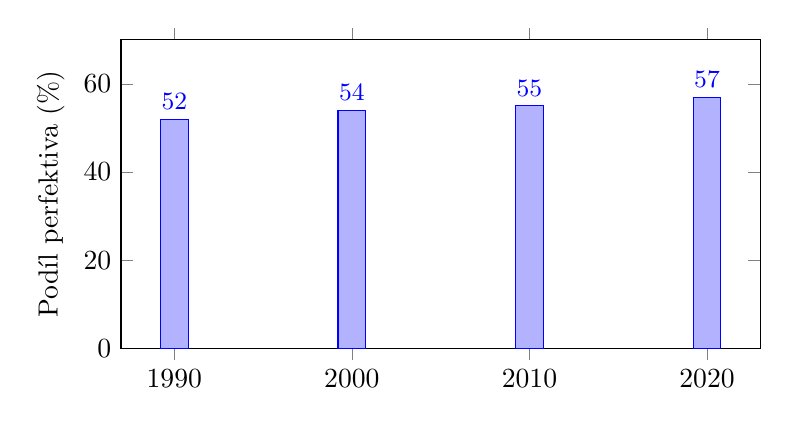
\begin{tikzpicture}
    \begin{axis}[ybar, width=.8\textwidth, height=5.5cm,
        symbolic x coords={1990,2000,2010,2020}, xtick=data,
        ylabel={Podíl perfektiva (\%)}, ymin=0, ymax=70,
        nodes near coords, every node near coord/.append style={font=\small}]
      \addplot coordinates {(1990,52) (2000,54) (2010,55) (2020,57)};
    \end{axis}
  \end{tikzpicture}
  \caption{Podíl perfektivních tvarů podle desetiletí (smyšlená data)}
  \label{fig:graf}
\end{figure}

\begin{figure}[htbp]
  \centering
  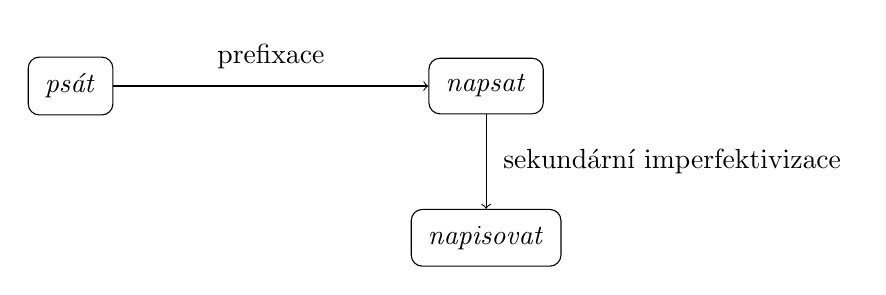
\begin{tikzpicture}[node distance=2.2cm, every node/.style={draw, rounded corners, inner sep=6pt}]
    \node (ipf) {\emph{psát}};
    \node (pf) [right=4cm of ipf] {\emph{napsat}};
    \node (sec) [below=1.2cm of pf] {\emph{napisovat}};
    \draw[->] (ipf) -- node[above, draw=none] {prefixace} (pf);
    \draw[->] (pf) -- node[right, draw=none] {sekundární imperfektivizace} (sec);
  \end{tikzpicture}
  \caption{Tvoření vidových dvojic}
  \label{fig:schema}
\end{figure}

\chapter{Závěr}
Text.

\thesisbibliography

\appendix
% Každá příloha je kapitola; jejich počet se uvádí v~abstraktu automaticky.
\chapter{Korpusová data}
\label{app:data}
\begin{table}[htbp]
  \centering
  \begin{tabular}{l l S[table-format=4.0] S[table-format=4.0]}
    \toprule
    {Imperfektivum} & {Perfektivum} & {ipf.} & {pf.} \\
    \midrule
    \emph{dělat}   & \emph{udělat}   & 2140 & 3120 \\
    \emph{psát}    & \emph{napsat}   & 1210 & 1530 \\
    \emph{říkat}   & \emph{říct}     & 1980 & 2650 \\
    \emph{kupovat} & \emph{koupit}   &  410 &  880 \\
    \bottomrule
  \end{tabular}
  \caption{Nejčastější vidové dvojice (smyšlená data)}
  \label{tab:dvojice}
\end{table}

\chapter{Seznam zkratek}
\label{app:zkratky}
\begin{tabular}{@{}ll@{}}
  \gm{acc} & akuzativ \\
  \gm{ger} & gerundium \\
  \gm{top} & topik \\
\end{tabular}

\end{document}
